\section{Singleton}

\subsection{Definition}
The singleton pattern is a software design pattern that restricts the instantiation of a class to one object. This is useful when exactly one object is needed to coordinate actions across the system.
\subsection{Role}
The pattern involves a single class which create and object like while making sure that only single object is created.
\subsection{Example}

The following Singleton pattern was found in the following instance: 'w.tools.explorer.model.Attri-
buteModelBuilder::singleton:fw.tools.explorer.model.AttributeModelBuilder'

\begin{center}
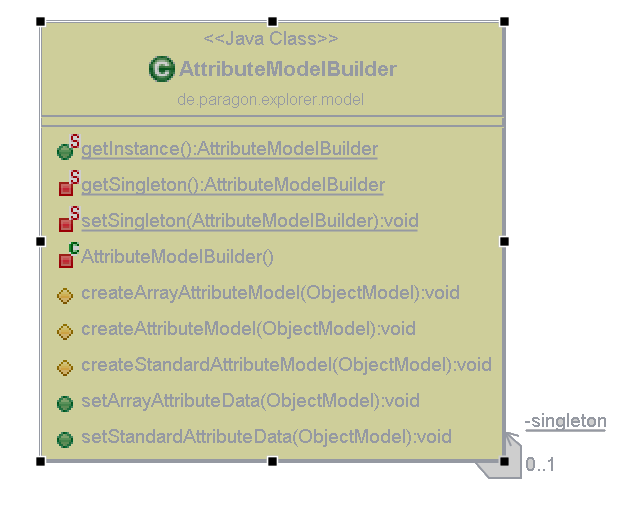
\includegraphics{Singleton}
\end{center}



In the function AttributeModelBuilder we can see the instance receiving the instance of an Object and we can see how it obtains a single object:

\begin{spverbatim}
public final class AttributeModelBuilder {
	private static AttributeModelBuilder	singleton;

	public static AttributeModelBuilder getInstance() {
		return AttributeModelBuilder.getSingleton();
	}
	private static AttributeModelBuilder getSingleton() {
		if (AttributeModelBuilder.singleton == null) {
			AttributeModelBuilder.setSingleton(new AttributeModelBuilder());
		}
		return AttributeModelBuilder.singleton;
	}
		private static void setSingleton(AttributeModelBuilder builder) {
		AttributeModelBuilder.singleton = builder;
	}
....}
\end{spverbatim}